\documentclass[a4paper]{article}

\usepackage{graphicx}
\usepackage{todonotes}

\begin{document}

\todo[inline]{title}
\todo[inline]{details}
\todo[inline]{abstract}

\section{Adder design, simulation and synthesis}
\label{sec:adder}

The adder was written from scratch as part of the \texttt{multiplier\_datapath} module. The source code for the adder is given by lines 69--72 of Listing~\ref{lst:multiplier-datapath}.

\subsection{Simulation of adder}
\label{sec:adder:sim}

The adder was not simulated on its own, but only as a part of \texttt{multiplier\_datapath} (see Section~\ref{sec:reg:sim}). \todo{finish}

\section{Register design, simulation and synthesis}
\label{seg:reg}

The registers were implemented in the \texttt{multiplier\_datapath} module, together with the adder/shifter. This module was written from scratch; the source code is given in Listing~\ref{lst:multiplier_datapath}.

The \texttt{multiplier\_datapath} module has two 4-bit data inputs, \texttt{multiplicand} and \texttt{multiplier}. These are the two input numbers to the multiplier, and are equivalent to \texttt{M} and \texttt{Qin} respectively in the sample code. Similarly, there is one 8-bit data output, \texttt{product}, which is equivalent to \texttt{AQ} in the sample code.

The module takes two control signals, \texttt{do\_init} and \texttt{do\_shift}, in addition to the clock and asynchronous reset signals. If \texttt{do\_init} is asserted during a rising clock edge, the \texttt{a} and \texttt{q} registers are loaded with their initial values (0 and \texttt{multiplier} respectively). If \texttt{do\_shift} is asserted during a rising clock edge, then \texttt{multiplicand} is conditionally added to \texttt{a}, and then \texttt{a} and \texttt{q} are shifted right by one place, completing one iteration of the multiplication algorithm in a single clock cycle.

\subsection{Simulation of registers}
\label{sec:reg:sim}

A testbench for the \texttt{multiplier\_datapath} module was prepared. Its source code is given in Listing~\ref{lst:test-multiplier-datapath}. The testbench was then simulated using ModelSim, giving the waveform diagram shown in Figure~\ref{fig:test-multiplier-datapath}. After correcting some minor syntax errors, the testbench and the module under test worked first time, without any assertions failing.

The testbench begins with the reset signal active, and checks that the registers \texttt{a} and \texttt{q} (whose values are concatenated to form the signal \texttt{product}) are reset to zero. It then releases the system from reset, and asserts the \texttt{do\_init} for one clock cycle, checking that \texttt{q} is set to 6, the value arbitrarily chosen for the second multiplier input. It then asserts \texttt{do\_shift} for four of the five following clock cycles, checking the state of the registers at each stage. The results of these operations can be observed in Figure~\ref{fig:test-multiplier-datapath}.

\begin{figure}[ht]
  \centering
  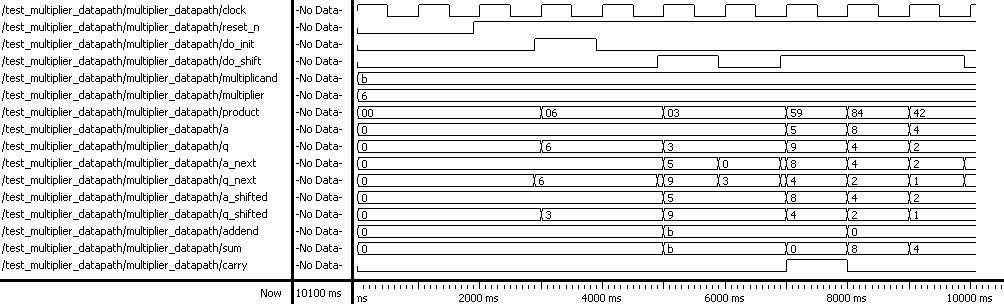
\includegraphics[width=\textwidth]{assets/test_multiplier_datapath}
  \caption{Waveform of the \texttt{test\_multiplier\_datapath} testbench.}
  \label{fig:test-multiplier-datapath}
\end{figure}

\end{document}
